\documentclass[1p]{elsarticle_modified}
%\bibliographystyle{elsarticle-num}

%\usepackage[colorlinks]{hyperref}
%\usepackage{abbrmath_seonhwa} %\Abb, \Ascr, \Acal ,\Abf, \Afrak
\usepackage{amsfonts}
\usepackage{amssymb}
\usepackage{amsmath}
\usepackage{amsthm}
\usepackage{scalefnt}
\usepackage{amsbsy}
\usepackage{kotex}
\usepackage{caption}
\usepackage{subfig}
\usepackage{color}
\usepackage{graphicx}
\usepackage{xcolor} %% white, black, red, green, blue, cyan, magenta, yellow
\usepackage{float}
\usepackage{setspace}
\usepackage{hyperref}

\usepackage{tikz}
\usetikzlibrary{arrows}

\usepackage{multirow}
\usepackage{array} % fixed length table
\usepackage{hhline}

%%%%%%%%%%%%%%%%%%%%%
\makeatletter
\renewcommand*\env@matrix[1][\arraystretch]{%
	\edef\arraystretch{#1}%
	\hskip -\arraycolsep
	\let\@ifnextchar\new@ifnextchar
	\array{*\c@MaxMatrixCols c}}
\makeatother %https://tex.stackexchange.com/questions/14071/how-can-i-increase-the-line-spacing-in-a-matrix
%%%%%%%%%%%%%%%

\usepackage[normalem]{ulem}

\newcommand{\msout}[1]{\ifmmode\text{\sout{\ensuremath{#1}}}\else\sout{#1}\fi}
%SOURCE: \msout is \stkout macro in https://tex.stackexchange.com/questions/20609/strikeout-in-math-mode

\newcommand{\cancel}[1]{
	\ifmmode
	{\color{red}\msout{#1}}
	\else
	{\color{red}\sout{#1}}
	\fi
}

\newcommand{\add}[1]{
	{\color{blue}\uwave{#1}}
}

\newcommand{\replace}[2]{
	\ifmmode
	{\color{red}\msout{#1}}{\color{blue}\uwave{#2}}
	\else
	{\color{red}\sout{#1}}{\color{blue}\uwave{#2}}
	\fi
}

\newcommand{\Sol}{\mathcal{S}} %segment
\newcommand{\D}{D} %diagram
\newcommand{\A}{\mathcal{A}} %arc


%%%%%%%%%%%%%%%%%%%%%%%%%%%%%5 test

\def\sl{\operatorname{\textup{SL}}(2,\Cbb)}
\def\psl{\operatorname{\textup{PSL}}(2,\Cbb)}
\def\quan{\mkern 1mu \triangleright \mkern 1mu}

\theoremstyle{definition}
\newtheorem{thm}{Theorem}[section]
\newtheorem{prop}[thm]{Proposition}
\newtheorem{lem}[thm]{Lemma}
\newtheorem{ques}[thm]{Question}
\newtheorem{cor}[thm]{Corollary}
\newtheorem{defn}[thm]{Definition}
\newtheorem{exam}[thm]{Example}
\newtheorem{rmk}[thm]{Remark}
\newtheorem{alg}[thm]{Algorithm}

\newcommand{\I}{\sqrt{-1}}
\begin{document}

%\begin{frontmatter}
%
%\title{Boundary parabolic representations of knots up to 8 crossings}
%
%%% Group authors per affiliation:
%\author{Yunhi Cho} 
%\address{Department of Mathematics, University of Seoul, Seoul, Korea}
%\ead{yhcho@uos.ac.kr}
%
%
%\author{Seonhwa Kim} %\fnref{s_kim}}
%\address{Center for Geometry and Physics, Institute for Basic Science, Pohang, 37673, Korea}
%\ead{ryeona17@ibs.re.kr}
%
%\author{Hyuk Kim}
%\address{Department of Mathematical Sciences, Seoul National University, Seoul 08826, Korea}
%\ead{hyukkim@snu.ac.kr}
%
%\author{Seokbeom Yoon}
%\address{Department of Mathematical Sciences, Seoul National University, Seoul, 08826,  Korea}
%\ead{sbyoon15@snu.ac.kr}
%
%\begin{abstract}
%We find all boundary parabolic representation of knots up to 8 crossings.
%
%\end{abstract}
%\begin{keyword}
%    \MSC[2010] 57M25 
%\end{keyword}
%
%\end{frontmatter}

%\linenumbers
%\tableofcontents
%
\newcommand\colored[1]{\textcolor{white}{\rule[-0.35ex]{0.8em}{1.4ex}}\kern-0.8em\color{red} #1}%
%\newcommand\colored[1]{\textcolor{white}{ #1}\kern-2.17ex	\textcolor{white}{ #1}\kern-1.81ex	\textcolor{white}{ #1}\kern-2.15ex\color{red}#1	}

{\Large $\underline{11n_{169}~(K11n_{169})}$}

\setlength{\tabcolsep}{10pt}
\renewcommand{\arraystretch}{1.6}
\vspace{1cm}\begin{tabular}{m{100pt}>{\centering\arraybackslash}m{274pt}}
\multirow{5}{120pt}{
	\centering
	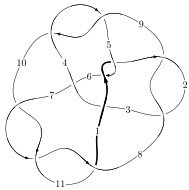
\includegraphics[width=112pt]{../../../GIT/diagram.site/Diagrams/png/785_11n_169.png}\\
\ \ \ A knot diagram\footnotemark}&
\allowdisplaybreaks
\textbf{Linearized knot diagam} \\
\cline{2-2}
 &
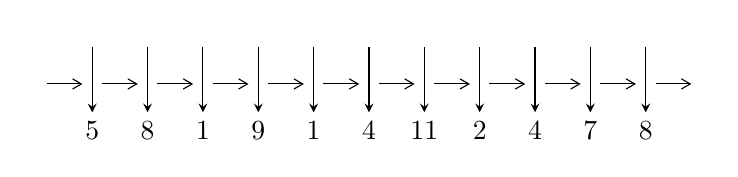
\begin{tikzpicture}[x=20pt, y=17pt]
	% nodes
	\node (C0) at (0, 0) {};
	\node (C1) at (1, 0) {};
	\node (C1U) at (1, +1) {};
	\node (C1D) at (1, -1) {5};

	\node (C2) at (2, 0) {};
	\node (C2U) at (2, +1) {};
	\node (C2D) at (2, -1) {8};

	\node (C3) at (3, 0) {};
	\node (C3U) at (3, +1) {};
	\node (C3D) at (3, -1) {1};

	\node (C4) at (4, 0) {};
	\node (C4U) at (4, +1) {};
	\node (C4D) at (4, -1) {9};

	\node (C5) at (5, 0) {};
	\node (C5U) at (5, +1) {};
	\node (C5D) at (5, -1) {1};

	\node (C6) at (6, 0) {};
	\node (C6U) at (6, +1) {};
	\node (C6D) at (6, -1) {4};

	\node (C7) at (7, 0) {};
	\node (C7U) at (7, +1) {};
	\node (C7D) at (7, -1) {11};

	\node (C8) at (8, 0) {};
	\node (C8U) at (8, +1) {};
	\node (C8D) at (8, -1) {2};

	\node (C9) at (9, 0) {};
	\node (C9U) at (9, +1) {};
	\node (C9D) at (9, -1) {4};

	\node (C10) at (10, 0) {};
	\node (C10U) at (10, +1) {};
	\node (C10D) at (10, -1) {7};

	\node (C11) at (11, 0) {};
	\node (C11U) at (11, +1) {};
	\node (C11D) at (11, -1) {8};
	\node (C12) at (12, 0) {};

	% arrows
	\draw[->,>={angle 60}]
	(C0) edge (C1) (C1) edge (C2) (C2) edge (C3) (C3) edge (C4) (C4) edge (C5) (C5) edge (C6) (C6) edge (C7) (C7) edge (C8) (C8) edge (C9) (C9) edge (C10) (C10) edge (C11) (C11) edge (C12) ;	\draw[->,>=stealth]
	(C1U) edge (C1D) (C2U) edge (C2D) (C3U) edge (C3D) (C4U) edge (C4D) (C5U) edge (C5D) (C6U) edge (C6D) (C7U) edge (C7D) (C8U) edge (C8D) (C9U) edge (C9D) (C10U) edge (C10D) (C11U) edge (C11D) ;
	\end{tikzpicture} \\
\hhline{~~} \\& 
\textbf{Solving Sequence} \\ \cline{2-2} 
 &
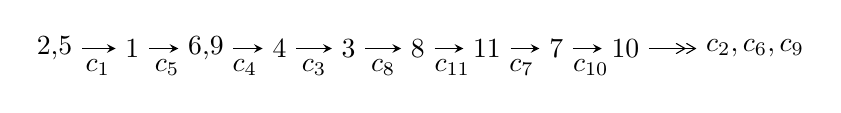
\begin{tikzpicture}[x=25pt, y=7pt]
	% node
	\node (A0) at (-1/8, 0) {2,5};
	\node (A1) at (1, 0) {1};
	\node (A2) at (33/16, 0) {6,9};
	\node (A3) at (25/8, 0) {4};
	\node (A4) at (33/8, 0) {3};
	\node (A5) at (41/8, 0) {8};
	\node (A6) at (49/8, 0) {11};
	\node (A7) at (57/8, 0) {7};
	\node (A8) at (65/8, 0) {10};
	\node (C1) at (1/2, -1) {$c_{1}$};
	\node (C2) at (3/2, -1) {$c_{5}$};
	\node (C3) at (21/8, -1) {$c_{4}$};
	\node (C4) at (29/8, -1) {$c_{3}$};
	\node (C5) at (37/8, -1) {$c_{8}$};
	\node (C6) at (45/8, -1) {$c_{11}$};
	\node (C7) at (53/8, -1) {$c_{7}$};
	\node (C8) at (61/8, -1) {$c_{10}$};
	\node (A9) at (10, 0) {$c_{2},c_{6},c_{9}$};

	% edge
	\draw[->,>=stealth]	
	(A0) edge (A1) (A1) edge (A2) (A2) edge (A3) (A3) edge (A4) (A4) edge (A5) (A5) edge (A6) (A6) edge (A7) (A7) edge (A8) ;
	\draw[->>,>={angle 60}]	
	(A8) edge (A9);
\end{tikzpicture} \\ 

\end{tabular} \\

\footnotetext{
The image of knot diagram is generated by the software ``\textbf{Draw programme}" developed by Andrew Bartholomew(\url{http://www.layer8.co.uk/maths/draw/index.htm\#Running-draw}), where we modified some parts for our purpose(\url{https://github.com/CATsTAILs/LinksPainter}).
}\phantom \\ \newline 
\centering \textbf{Ideals for irreducible components\footnotemark of $X_{\text{par}}$} 
 
\begin{align*}
I^u_{1}&=\langle 
- u^{12}+8 u^{11}+\cdots+4 b-12,\;3 u^{12}-22 u^{11}+\cdots+8 a+36,\;u^{13}-8 u^{12}+\cdots+56 u-8\rangle \\
I^u_{2}&=\langle 
u^5+u^4+u^3- u^2+b-1,\;u^7+u^6+2 u^5+2 u^3-2 u^2+a-2,\;u^8+u^7+2 u^6- u^5+u^4-3 u^3+u^2-2 u+1\rangle \\
I^u_{3}&=\langle 
-5 a^5 u-4 a^5+7 a^4+5 a^3 u+4 a^3+8 a^2 u-2 a^2-6 a u+7 b+5 a-3 u-1,\\
\phantom{I^u_{3}}&\phantom{= \langle  }a^6+a^5 u- a^4-3 a^3 u-2 a^3+3 a^2 u+a^2+2 a u+3 a-3 u-1,\;u^2+u+1\rangle \\
\\
\end{align*}
\raggedright * 3 irreducible components of $\dim_{\mathbb{C}}=0$, with total 33 representations.\\
\footnotetext{All coefficients of polynomials are rational numbers. But the coefficients are sometimes approximated in decimal forms when there is not enough margin.}
\newpage
\renewcommand{\arraystretch}{1}
\centering \section*{I. $I^u_{1}= \langle - u^{12}+8 u^{11}+\cdots+4 b-12,\;3 u^{12}-22 u^{11}+\cdots+8 a+36,\;u^{13}-8 u^{12}+\cdots+56 u-8 \rangle$}
\flushleft \textbf{(i) Arc colorings}\\
\begin{tabular}{m{7pt} m{180pt} m{7pt} m{180pt} }
\flushright $a_{2}=$&$\begin{pmatrix}1\\0\end{pmatrix}$ \\
\flushright $a_{5}=$&$\begin{pmatrix}0\\u\end{pmatrix}$ \\
\flushright $a_{1}=$&$\begin{pmatrix}1\\- u^2\end{pmatrix}$ \\
\flushright $a_{6}=$&$\begin{pmatrix}- u\\u^3+u\end{pmatrix}$ \\
\flushright $a_{9}=$&$\begin{pmatrix}-\frac{3}{8} u^{12}+\frac{11}{4} u^{11}+\cdots+20 u-\frac{9}{2}\\\frac{1}{4} u^{12}-2 u^{11}+\cdots-\frac{33}{2} u+3\end{pmatrix}$ \\
\flushright $a_{4}=$&$\begin{pmatrix}\frac{1}{4} u^{12}-2 u^{11}+\cdots-13 u+\frac{5}{2}\\\frac{1}{2} u^{11}-3 u^{10}+\cdots+\frac{25}{2} u-2\end{pmatrix}$ \\
\flushright $a_{3}=$&$\begin{pmatrix}-\frac{1}{4} u^{12}+\frac{3}{2} u^{11}+\cdots+\frac{3}{2} u+\frac{1}{2}\\-\frac{1}{2} u^{11}+3 u^{10}+\cdots-\frac{23}{2} u+2\end{pmatrix}$ \\
\flushright $a_{8}=$&$\begin{pmatrix}-\frac{1}{8} u^{12}+\frac{3}{4} u^{11}+\cdots+\frac{7}{2} u-\frac{3}{2}\\\frac{1}{4} u^{12}-2 u^{11}+\cdots-\frac{33}{2} u+3\end{pmatrix}$ \\
\flushright $a_{11}=$&$\begin{pmatrix}\frac{1}{4} u^{12}-2 u^{11}+\cdots-14 u+\frac{7}{2}\\\frac{1}{2} u^{12}-\frac{7}{2} u^{11}+\cdots-\frac{29}{2} u+2\end{pmatrix}$ \\
\flushright $a_{7}=$&$\begin{pmatrix}u^{12}-\frac{27}{4} u^{11}+\cdots-\frac{73}{4} u+2\\-\frac{3}{4} u^{12}+\frac{11}{2} u^{11}+\cdots+29 u-4\end{pmatrix}$ \\
\flushright $a_{10}=$&$\begin{pmatrix}-\frac{1}{4} u^{12}+\frac{5}{4} u^{11}+\cdots-\frac{55}{4} u+4\\\frac{3}{4} u^{12}-\frac{11}{2} u^{11}+\cdots-29 u+4\end{pmatrix}$\\ \flushright $a_{10}=$&$\begin{pmatrix}-\frac{1}{4} u^{12}+\frac{5}{4} u^{11}+\cdots-\frac{55}{4} u+4\\\frac{3}{4} u^{12}-\frac{11}{2} u^{11}+\cdots-29 u+4\end{pmatrix}$\\&\end{tabular}
\flushleft \textbf{(ii) Obstruction class $= -1$}\\~\\
\flushleft \textbf{(iii) Cusp Shapes $= - u^{12}+5 u^{11}-15 u^{10}+31 u^9-51 u^8+70 u^7-85 u^6+89 u^5-83 u^4+63 u^3-43 u^2+24 u-22$}\\~\\
\newpage\renewcommand{\arraystretch}{1}
\flushleft \textbf{(iv) u-Polynomials at the component}\newline \\
\begin{tabular}{m{50pt}|m{274pt}}
Crossings & \hspace{64pt}u-Polynomials at each crossing \\
\hline $$\begin{aligned}c_{1},c_{5}\end{aligned}$$&$\begin{aligned}
&u^{13}+8 u^{12}+\cdots+56 u+8
\end{aligned}$\\
\hline $$\begin{aligned}c_{2},c_{4},c_{8}\\c_{9}\end{aligned}$$&$\begin{aligned}
&u^{13}+3 u^{11}+\cdots+2 u+1
\end{aligned}$\\
\hline $$\begin{aligned}c_{3},c_{6}\end{aligned}$$&$\begin{aligned}
&u^{13}-2 u^{12}+\cdots-4 u+1
\end{aligned}$\\
\hline $$\begin{aligned}c_{7},c_{10},c_{11}\end{aligned}$$&$\begin{aligned}
&u^{13}+6 u^{12}+\cdots+14 u+4
\end{aligned}$\\
\hline
\end{tabular}\\~\\
\newpage\renewcommand{\arraystretch}{1}
\flushleft \textbf{(v) Riley Polynomials at the component}\newline \\
\begin{tabular}{m{50pt}|m{274pt}}
Crossings & \hspace{64pt}Riley Polynomials at each crossing \\
\hline $$\begin{aligned}c_{1},c_{5}\end{aligned}$$&$\begin{aligned}
&y^{13}+4 y^{12}+\cdots+480 y-64
\end{aligned}$\\
\hline $$\begin{aligned}c_{2},c_{4},c_{8}\\c_{9}\end{aligned}$$&$\begin{aligned}
&y^{13}+6 y^{12}+\cdots+2 y-1
\end{aligned}$\\
\hline $$\begin{aligned}c_{3},c_{6}\end{aligned}$$&$\begin{aligned}
&y^{13}-26 y^{12}+\cdots+42 y-1
\end{aligned}$\\
\hline $$\begin{aligned}c_{7},c_{10},c_{11}\end{aligned}$$&$\begin{aligned}
&y^{13}-16 y^{12}+\cdots+204 y-16
\end{aligned}$\\
\hline
\end{tabular}\\~\\
\newpage\flushleft \textbf{(vi) Complex Volumes and Cusp Shapes}
$$\begin{array}{c|c|c}  
\text{Solutions to }I^u_{1}& \I (\text{vol} + \sqrt{-1}CS) & \text{Cusp shape}\\
 \hline 
\begin{aligned}
u &= -0.326542 + 1.020100 I \\
a &= -0.503264 + 0.483746 I \\
b &= \phantom{-}0.329129 + 0.671341 I\end{aligned}
 & -1.07131 + 1.81105 I & -12.48073 - 2.50977 I \\ \hline\begin{aligned}
u &= -0.326542 - 1.020100 I \\
a &= -0.503264 - 0.483746 I \\
b &= \phantom{-}0.329129 - 0.671341 I\end{aligned}
 & -1.07131 - 1.81105 I & -12.48073 + 2.50977 I \\ \hline\begin{aligned}
u &= \phantom{-}1.161480 + 0.385396 I \\
a &= \phantom{-}0.216539 - 0.581687 I \\
b &= -0.475687 + 0.592166 I\end{aligned}
 & -3.17225 + 0.94602 I & -12.22572 - 6.14642 I \\ \hline\begin{aligned}
u &= \phantom{-}1.161480 - 0.385396 I \\
a &= \phantom{-}0.216539 + 0.581687 I \\
b &= -0.475687 - 0.592166 I\end{aligned}
 & -3.17225 - 0.94602 I & -12.22572 + 6.14642 I \\ \hline\begin{aligned}
u &= \phantom{-}0.270743 + 1.206070 I \\
a &= \phantom{-}0.733128 - 0.331803 I \\
b &= -0.598666 - 0.794370 I\end{aligned}
 & \phantom{-}2.89440 - 2.21633 I & -9.35734 + 3.25180 I \\ \hline\begin{aligned}
u &= \phantom{-}0.270743 - 1.206070 I \\
a &= \phantom{-}0.733128 + 0.331803 I \\
b &= -0.598666 + 0.794370 I\end{aligned}
 & \phantom{-}2.89440 + 2.21633 I & -9.35734 - 3.25180 I \\ \hline\begin{aligned}
u &= \phantom{-}0.63465 + 1.27236 I \\
a &= -0.928004 + 0.162795 I \\
b &= \phantom{-}0.796089 + 1.077430 I\end{aligned}
 & -0.15730 - 7.29804 I & -11.37128 + 6.48312 I \\ \hline\begin{aligned}
u &= \phantom{-}0.63465 - 1.27236 I \\
a &= -0.928004 - 0.162795 I \\
b &= \phantom{-}0.796089 - 1.077430 I\end{aligned}
 & -0.15730 + 7.29804 I & -11.37128 - 6.48312 I \\ \hline\begin{aligned}
u &= \phantom{-}1.26554 + 0.69993 I \\
a &= -0.057804 + 0.864578 I \\
b &= \phantom{-}0.678296 - 1.053700 I\end{aligned}
 & -11.99570 + 3.34885 I & -12.69425 - 2.28469 I \\ \hline\begin{aligned}
u &= \phantom{-}1.26554 - 0.69993 I \\
a &= -0.057804 - 0.864578 I \\
b &= \phantom{-}0.678296 + 1.053700 I\end{aligned}
 & -11.99570 - 3.34885 I & -12.69425 + 2.28469 I\\
 \hline 
 \end{array}$$\newpage$$\begin{array}{c|c|c}  
\text{Solutions to }I^u_{1}& \I (\text{vol} + \sqrt{-1}CS) & \text{Cusp shape}\\
 \hline 
\begin{aligned}
u &= \phantom{-}0.83155 + 1.23498 I \\
a &= \phantom{-}1.136480 + 0.017597 I \\
b &= -0.92331 - 1.41816 I\end{aligned}
 & -10.0617 - 10.8173 I & -12.24076 + 5.20880 I \\ \hline\begin{aligned}
u &= \phantom{-}0.83155 - 1.23498 I \\
a &= \phantom{-}1.136480 - 0.017597 I \\
b &= -0.92331 + 1.41816 I\end{aligned}
 & -10.0617 + 10.8173 I & -12.24076 - 5.20880 I \\ \hline\begin{aligned}
u &= \phantom{-}0.325158\phantom{ +0.000000I} \\
a &= -1.19415\phantom{ +0.000000I} \\
b &= \phantom{-}0.388289\phantom{ +0.000000I}\end{aligned}
 & -0.575325\phantom{ +0.000000I} & -17.2600\phantom{ +0.000000I}\\
 \hline 
 \end{array}$$\newpage\newpage\renewcommand{\arraystretch}{1}
\centering \section*{II. $I^u_{2}= \langle u^5+u^4+u^3- u^2+b-1,\;u^7+u^6+2 u^5+2 u^3-2 u^2+a-2,\;u^8+u^7+2 u^6- u^5+u^4-3 u^3+u^2-2 u+1 \rangle$}
\flushleft \textbf{(i) Arc colorings}\\
\begin{tabular}{m{7pt} m{180pt} m{7pt} m{180pt} }
\flushright $a_{2}=$&$\begin{pmatrix}1\\0\end{pmatrix}$ \\
\flushright $a_{5}=$&$\begin{pmatrix}0\\u\end{pmatrix}$ \\
\flushright $a_{1}=$&$\begin{pmatrix}1\\- u^2\end{pmatrix}$ \\
\flushright $a_{6}=$&$\begin{pmatrix}- u\\u^3+u\end{pmatrix}$ \\
\flushright $a_{9}=$&$\begin{pmatrix}- u^7- u^6-2 u^5-2 u^3+2 u^2+2\\- u^5- u^4- u^3+u^2+1\end{pmatrix}$ \\
\flushright $a_{4}=$&$\begin{pmatrix}- u^7-2 u^6-3 u^5- u^4+2 u^2+2 u+1\\- u^7- u^6-2 u^5+u^4- u^3+3 u^2+1\end{pmatrix}$ \\
\flushright $a_{3}=$&$\begin{pmatrix}-2 u^7-3 u^6-5 u^5- u^3+5 u^2+u+3\\- u^7- u^6-2 u^5+u^4- u^3+3 u^2- u+1\end{pmatrix}$ \\
\flushright $a_{8}=$&$\begin{pmatrix}- u^7- u^6-3 u^5- u^4-3 u^3+3 u^2+3\\- u^5- u^4- u^3+u^2+1\end{pmatrix}$ \\
\flushright $a_{11}=$&$\begin{pmatrix}3 u^7+4 u^6+7 u^5- u^4+2 u^3-7 u^2+u-4\\u^7+u^6+2 u^5- u^4+u^3-3 u^2+u-2\end{pmatrix}$ \\
\flushright $a_{7}=$&$\begin{pmatrix}u^7+2 u^6+4 u^5+2 u^4+2 u^3-3 u^2-2 u-4\\u^7+2 u^6+3 u^5+u^4+u^3-2 u^2- u-2\end{pmatrix}$ \\
\flushright $a_{10}=$&$\begin{pmatrix}-2 u^7-3 u^6-5 u^5-2 u^3+4 u^2+4\\- u^7-2 u^6-3 u^5- u^4- u^3+2 u^2+u+2\end{pmatrix}$\\ \flushright $a_{10}=$&$\begin{pmatrix}-2 u^7-3 u^6-5 u^5-2 u^3+4 u^2+4\\- u^7-2 u^6-3 u^5- u^4- u^3+2 u^2+u+2\end{pmatrix}$\\&\end{tabular}
\flushleft \textbf{(ii) Obstruction class $= 1$}\\~\\
\flushleft \textbf{(iii) Cusp Shapes $= 3 u^7+2 u^6+4 u^5-3 u^4+3 u^3-7 u^2- u-11$}\\~\\
\newpage\renewcommand{\arraystretch}{1}
\flushleft \textbf{(iv) u-Polynomials at the component}\newline \\
\begin{tabular}{m{50pt}|m{274pt}}
Crossings & \hspace{64pt}u-Polynomials at each crossing \\
\hline $$\begin{aligned}c_{1}\end{aligned}$$&$\begin{aligned}
&u^8+u^7+2 u^6- u^5+u^4-3 u^3+u^2-2 u+1
\end{aligned}$\\
\hline $$\begin{aligned}c_{2},c_{9}\end{aligned}$$&$\begin{aligned}
&u^8+3 u^6- u^5+3 u^4-3 u^3-3 u-1
\end{aligned}$\\
\hline $$\begin{aligned}c_{3},c_{6}\end{aligned}$$&$\begin{aligned}
&u^8+2 u^7+u^6+3 u^5+u^4+u^3+2 u^2- u+1
\end{aligned}$\\
\hline $$\begin{aligned}c_{4},c_{8}\end{aligned}$$&$\begin{aligned}
&u^8+3 u^6+u^5+3 u^4+3 u^3+3 u-1
\end{aligned}$\\
\hline $$\begin{aligned}c_{5}\end{aligned}$$&$\begin{aligned}
&u^8- u^7+2 u^6+u^5+u^4+3 u^3+u^2+2 u+1
\end{aligned}$\\
\hline $$\begin{aligned}c_{7}\end{aligned}$$&$\begin{aligned}
&u^8+u^7-5 u^6-4 u^5+8 u^4+5 u^3-3 u^2- u-1
\end{aligned}$\\
\hline $$\begin{aligned}c_{10},c_{11}\end{aligned}$$&$\begin{aligned}
&u^8- u^7-5 u^6+4 u^5+8 u^4-5 u^3-3 u^2+u-1
\end{aligned}$\\
\hline
\end{tabular}\\~\\
\newpage\renewcommand{\arraystretch}{1}
\flushleft \textbf{(v) Riley Polynomials at the component}\newline \\
\begin{tabular}{m{50pt}|m{274pt}}
Crossings & \hspace{64pt}Riley Polynomials at each crossing \\
\hline $$\begin{aligned}c_{1},c_{5}\end{aligned}$$&$\begin{aligned}
&y^8+3 y^7+8 y^6+11 y^5+5 y^4-7 y^3-9 y^2-2 y+1
\end{aligned}$\\
\hline $$\begin{aligned}c_{2},c_{4},c_{8}\\c_{9}\end{aligned}$$&$\begin{aligned}
&y^8+6 y^7+15 y^6+17 y^5+y^4-21 y^3-24 y^2-9 y+1
\end{aligned}$\\
\hline $$\begin{aligned}c_{3},c_{6}\end{aligned}$$&$\begin{aligned}
&y^8-2 y^7-9 y^6-7 y^5+5 y^4+11 y^3+8 y^2+3 y+1
\end{aligned}$\\
\hline $$\begin{aligned}c_{7},c_{10},c_{11}\end{aligned}$$&$\begin{aligned}
&y^8-11 y^7+49 y^6-112 y^5+134 y^4-71 y^3+3 y^2+5 y+1
\end{aligned}$\\
\hline
\end{tabular}\\~\\
\newpage\flushleft \textbf{(vi) Complex Volumes and Cusp Shapes}
$$\begin{array}{c|c|c}  
\text{Solutions to }I^u_{2}& \I (\text{vol} + \sqrt{-1}CS) & \text{Cusp shape}\\
 \hline 
\begin{aligned}
u &= \phantom{-}0.163169 + 0.915412 I \\
a &= \phantom{-}1.000040 + 0.736649 I \\
b &= -0.511162 + 1.035650 I\end{aligned}
 & -0.155635 - 0.787051 I & -8.59786 - 1.33483 I \\ \hline\begin{aligned}
u &= \phantom{-}0.163169 - 0.915412 I \\
a &= \phantom{-}1.000040 - 0.736649 I \\
b &= -0.511162 - 1.035650 I\end{aligned}
 & -0.155635 + 0.787051 I & -8.59786 + 1.33483 I \\ \hline\begin{aligned}
u &= \phantom{-}0.918626\phantom{ +0.000000I} \\
a &= -0.323992\phantom{ +0.000000I} \\
b &= -0.297628\phantom{ +0.000000I}\end{aligned}
 & -2.98361\phantom{ +0.000000I} & -12.1620\phantom{ +0.000000I} \\ \hline\begin{aligned}
u &= -0.404913 + 1.017880 I \\
a &= -1.143500 + 0.110127 I \\
b &= \phantom{-}0.350924 - 1.208540 I\end{aligned}
 & \phantom{-}5.21920 + 1.77211 I & -2.23409 - 0.85548 I \\ \hline\begin{aligned}
u &= -0.404913 - 1.017880 I \\
a &= -1.143500 - 0.110127 I \\
b &= \phantom{-}0.350924 + 1.208540 I\end{aligned}
 & \phantom{-}5.21920 - 1.77211 I & -2.23409 + 0.85548 I \\ \hline\begin{aligned}
u &= -0.95744 + 1.12705 I \\
a &= \phantom{-}0.720153 - 0.424011 I \\
b &= -0.211625 + 1.217620 I\end{aligned}
 & \phantom{-}1.24083 + 3.75870 I & -10.69968 - 3.38204 I \\ \hline\begin{aligned}
u &= -0.95744 - 1.12705 I \\
a &= \phantom{-}0.720153 + 0.424011 I \\
b &= -0.211625 - 1.217620 I\end{aligned}
 & \phantom{-}1.24083 - 3.75870 I & -10.69968 + 3.38204 I \\ \hline\begin{aligned}
u &= \phantom{-}0.479751\phantom{ +0.000000I} \\
a &= \phantom{-}2.17061\phantom{ +0.000000I} \\
b &= \phantom{-}1.04135\phantom{ +0.000000I}\end{aligned}
 & -12.9150\phantom{ +0.000000I} & -12.7750\phantom{ +0.000000I}\\
 \hline 
 \end{array}$$\newpage\newpage\renewcommand{\arraystretch}{1}
\centering \section*{III. $I^u_{3}= \langle -5 a^5 u+5 a^3 u+\cdots+5 a-1,\;a^5 u-3 a^3 u+\cdots+3 a-1,\;u^2+u+1 \rangle$}
\flushleft \textbf{(i) Arc colorings}\\
\begin{tabular}{m{7pt} m{180pt} m{7pt} m{180pt} }
\flushright $a_{2}=$&$\begin{pmatrix}1\\0\end{pmatrix}$ \\
\flushright $a_{5}=$&$\begin{pmatrix}0\\u\end{pmatrix}$ \\
\flushright $a_{1}=$&$\begin{pmatrix}1\\u+1\end{pmatrix}$ \\
\flushright $a_{6}=$&$\begin{pmatrix}- u\\u+1\end{pmatrix}$ \\
\flushright $a_{9}=$&$\begin{pmatrix}a\\\frac{5}{7} a^5 u-\frac{5}{7} a^3 u+\cdots-\frac{5}{7} a+\frac{1}{7}\end{pmatrix}$ \\
\flushright $a_{4}=$&$\begin{pmatrix}a^2 u\\-\frac{3}{7} a^5 u-\frac{4}{7} a^3 u+\cdots+\frac{10}{7} a-\frac{2}{7}\end{pmatrix}$ \\
\flushright $a_{3}=$&$\begin{pmatrix}-\frac{3}{7} a^5 u-\frac{4}{7} a^3 u+\cdots+\frac{10}{7} a-\frac{2}{7}\\-\frac{4}{7} a^5 u-\frac{3}{7} a^3 u+\cdots+\frac{11}{7} a+\frac{2}{7}\end{pmatrix}$ \\
\flushright $a_{8}=$&$\begin{pmatrix}\frac{5}{7} a^5 u-\frac{5}{7} a^3 u+\cdots+\frac{2}{7} a+\frac{1}{7}\\\frac{5}{7} a^5 u-\frac{5}{7} a^3 u+\cdots-\frac{5}{7} a+\frac{1}{7}\end{pmatrix}$ \\
\flushright $a_{11}=$&$\begin{pmatrix}a^2 u-2 u\\\frac{3}{7} a^5 u+\frac{4}{7} a^3 u+\cdots-\frac{10}{7} a+\frac{2}{7}\end{pmatrix}$ \\
\flushright $a_{7}=$&$\begin{pmatrix}-\frac{2}{7} a^5 u+a^4 u+\cdots+\frac{2}{7} a+\frac{8}{7}\\- a^4 u- a^4+a^3+a u+2\end{pmatrix}$ \\
\flushright $a_{10}=$&$\begin{pmatrix}a^3 u+a^3- a\\-\frac{4}{7} a^5 u- a^4 u+\cdots+\frac{4}{7} a+\frac{2}{7}\end{pmatrix}$\\ \flushright $a_{10}=$&$\begin{pmatrix}a^3 u+a^3- a\\-\frac{4}{7} a^5 u- a^4 u+\cdots+\frac{4}{7} a+\frac{2}{7}\end{pmatrix}$\\&\end{tabular}
\flushleft \textbf{(ii) Obstruction class $= -1$}\\~\\
\flushleft \textbf{(iii) Cusp Shapes $= -4 u-14$}\\~\\
\newpage\renewcommand{\arraystretch}{1}
\flushleft \textbf{(iv) u-Polynomials at the component}\newline \\
\begin{tabular}{m{50pt}|m{274pt}}
Crossings & \hspace{64pt}u-Polynomials at each crossing \\
\hline $$\begin{aligned}c_{1},c_{5}\end{aligned}$$&$\begin{aligned}
&(u^2- u+1)^6
\end{aligned}$\\
\hline $$\begin{aligned}c_{2},c_{4},c_{8}\\c_{9}\end{aligned}$$&$\begin{aligned}
&u^{12}- u^{11}+\cdots+14 u+7
\end{aligned}$\\
\hline $$\begin{aligned}c_{3},c_{6}\end{aligned}$$&$\begin{aligned}
&u^{12}- u^{11}+\cdots-56 u+13
\end{aligned}$\\
\hline $$\begin{aligned}c_{7},c_{10},c_{11}\end{aligned}$$&$\begin{aligned}
&(u^3- u^2-2 u+1)^4
\end{aligned}$\\
\hline
\end{tabular}\\~\\
\newpage\renewcommand{\arraystretch}{1}
\flushleft \textbf{(v) Riley Polynomials at the component}\newline \\
\begin{tabular}{m{50pt}|m{274pt}}
Crossings & \hspace{64pt}Riley Polynomials at each crossing \\
\hline $$\begin{aligned}c_{1},c_{5}\end{aligned}$$&$\begin{aligned}
&(y^2+y+1)^6
\end{aligned}$\\
\hline $$\begin{aligned}c_{2},c_{4},c_{8}\\c_{9}\end{aligned}$$&$\begin{aligned}
&y^{12}+3 y^{11}+\cdots-140 y^2+49
\end{aligned}$\\
\hline $$\begin{aligned}c_{3},c_{6}\end{aligned}$$&$\begin{aligned}
&y^{12}-13 y^{11}+\cdots-432 y+169
\end{aligned}$\\
\hline $$\begin{aligned}c_{7},c_{10},c_{11}\end{aligned}$$&$\begin{aligned}
&(y^3-5 y^2+6 y-1)^4
\end{aligned}$\\
\hline
\end{tabular}\\~\\
\newpage\flushleft \textbf{(vi) Complex Volumes and Cusp Shapes}
$$\begin{array}{c|c|c}  
\text{Solutions to }I^u_{3}& \I (\text{vol} + \sqrt{-1}CS) & \text{Cusp shape}\\
 \hline 
\begin{aligned}
u &= -0.500000 + 0.866025 I \\
a &= -1.100660 + 0.111510 I \\
b &= \phantom{-}0.231240 - 1.394380 I\end{aligned}
 & \phantom{-}4.22983 + 2.02988 I & -12.00000 - 3.46410 I \\ \hline\begin{aligned}
u &= -0.500000 + 0.866025 I \\
a &= \phantom{-}1.091430 + 0.189362 I \\
b &= -1.61068 - 0.71000 I\end{aligned}
 & -12.68950 + 2.02988 I & -12.00000 - 3.46410 I \\ \hline\begin{aligned}
u &= -0.500000 + 0.866025 I \\
a &= -1.045080 + 0.441811 I \\
b &= \phantom{-}0.763411 - 0.046058 I\end{aligned}
 & -1.40994 + 2.02988 I & -12.00000 - 3.46410 I \\ \hline\begin{aligned}
u &= -0.500000 + 0.866025 I \\
a &= \phantom{-}0.421593 + 0.638105 I \\
b &= -0.139922 + 1.125970 I\end{aligned}
 & -1.40994 + 2.02988 I & -12.00000 - 3.46410 I \\ \hline\begin{aligned}
u &= -0.500000 + 0.866025 I \\
a &= \phantom{-}1.323190 - 0.496928 I \\
b &= -0.453761 + 1.008960 I\end{aligned}
 & \phantom{-}4.22983 + 2.02988 I & -12.00000 - 3.46410 I \\ \hline\begin{aligned}
u &= -0.500000 + 0.866025 I \\
a &= -0.19046 - 1.74989 I \\
b &= \phantom{-}0.709707 - 0.850523 I\end{aligned}
 & -12.68950 + 2.02988 I & -12.00000 - 3.46410 I \\ \hline\begin{aligned}
u &= -0.500000 - 0.866025 I \\
a &= -1.100660 - 0.111510 I \\
b &= \phantom{-}0.231240 + 1.394380 I\end{aligned}
 & \phantom{-}4.22983 - 2.02988 I & -12.00000 + 3.46410 I \\ \hline\begin{aligned}
u &= -0.500000 - 0.866025 I \\
a &= \phantom{-}1.091430 - 0.189362 I \\
b &= -1.61068 + 0.71000 I\end{aligned}
 & -12.68950 - 2.02988 I & -12.00000 + 3.46410 I \\ \hline\begin{aligned}
u &= -0.500000 - 0.866025 I \\
a &= -1.045080 - 0.441811 I \\
b &= \phantom{-}0.763411 + 0.046058 I\end{aligned}
 & -1.40994 - 2.02988 I & -12.00000 + 3.46410 I \\ \hline\begin{aligned}
u &= -0.500000 - 0.866025 I \\
a &= \phantom{-}0.421593 - 0.638105 I \\
b &= -0.139922 - 1.125970 I\end{aligned}
 & -1.40994 - 2.02988 I & -12.00000 + 3.46410 I\\
 \hline 
 \end{array}$$\newpage$$\begin{array}{c|c|c}  
\text{Solutions to }I^u_{3}& \I (\text{vol} + \sqrt{-1}CS) & \text{Cusp shape}\\
 \hline 
\begin{aligned}
u &= -0.500000 - 0.866025 I \\
a &= \phantom{-}1.323190 + 0.496928 I \\
b &= -0.453761 - 1.008960 I\end{aligned}
 & \phantom{-}4.22983 - 2.02988 I & -12.00000 + 3.46410 I \\ \hline\begin{aligned}
u &= -0.500000 - 0.866025 I \\
a &= -0.19046 + 1.74989 I \\
b &= \phantom{-}0.709707 + 0.850523 I\end{aligned}
 & -12.68950 - 2.02988 I & -12.00000 + 3.46410 I\\
 \hline 
 \end{array}$$\newpage
\newpage\renewcommand{\arraystretch}{1}
\centering \section*{ IV. u-Polynomials}
\begin{tabular}{m{50pt}|m{274pt}}
Crossings & \hspace{64pt}u-Polynomials at each crossing \\
\hline $$\begin{aligned}c_{1}\end{aligned}$$&$\begin{aligned}
&(u^2- u+1)^6(u^8+u^7+2 u^6- u^5+u^4-3 u^3+u^2-2 u+1)\\
&\cdot(u^{13}+8 u^{12}+\cdots+56 u+8)
\end{aligned}$\\
\hline $$\begin{aligned}c_{2},c_{9}\end{aligned}$$&$\begin{aligned}
&(u^8+3 u^6- u^5+3 u^4-3 u^3-3 u-1)(u^{12}- u^{11}+\cdots+14 u+7)\\
&\cdot(u^{13}+3 u^{11}+\cdots+2 u+1)
\end{aligned}$\\
\hline $$\begin{aligned}c_{3},c_{6}\end{aligned}$$&$\begin{aligned}
&(u^8+2 u^7+\cdots- u+1)(u^{12}- u^{11}+\cdots-56 u+13)\\
&\cdot(u^{13}-2 u^{12}+\cdots-4 u+1)
\end{aligned}$\\
\hline $$\begin{aligned}c_{4},c_{8}\end{aligned}$$&$\begin{aligned}
&(u^8+3 u^6+u^5+3 u^4+3 u^3+3 u-1)(u^{12}- u^{11}+\cdots+14 u+7)\\
&\cdot(u^{13}+3 u^{11}+\cdots+2 u+1)
\end{aligned}$\\
\hline $$\begin{aligned}c_{5}\end{aligned}$$&$\begin{aligned}
&(u^2- u+1)^6(u^8- u^7+2 u^6+u^5+u^4+3 u^3+u^2+2 u+1)\\
&\cdot(u^{13}+8 u^{12}+\cdots+56 u+8)
\end{aligned}$\\
\hline $$\begin{aligned}c_{7}\end{aligned}$$&$\begin{aligned}
&(u^3- u^2-2 u+1)^4(u^8+u^7-5 u^6-4 u^5+8 u^4+5 u^3-3 u^2- u-1)\\
&\cdot(u^{13}+6 u^{12}+\cdots+14 u+4)
\end{aligned}$\\
\hline $$\begin{aligned}c_{10},c_{11}\end{aligned}$$&$\begin{aligned}
&(u^3- u^2-2 u+1)^4(u^8- u^7-5 u^6+4 u^5+8 u^4-5 u^3-3 u^2+u-1)\\
&\cdot(u^{13}+6 u^{12}+\cdots+14 u+4)
\end{aligned}$\\
\hline
\end{tabular}\newpage\renewcommand{\arraystretch}{1}
\centering \section*{ V. Riley Polynomials}
\begin{tabular}{m{50pt}|m{274pt}}
Crossings & \hspace{64pt}Riley Polynomials at each crossing \\
\hline $$\begin{aligned}c_{1},c_{5}\end{aligned}$$&$\begin{aligned}
&(y^2+y+1)^6(y^8+3 y^7+8 y^6+11 y^5+5 y^4-7 y^3-9 y^2-2 y+1)\\
&\cdot(y^{13}+4 y^{12}+\cdots+480 y-64)
\end{aligned}$\\
\hline $$\begin{aligned}c_{2},c_{4},c_{8}\\c_{9}\end{aligned}$$&$\begin{aligned}
&(y^8+6 y^7+15 y^6+17 y^5+y^4-21 y^3-24 y^2-9 y+1)\\
&\cdot(y^{12}+3 y^{11}+\cdots-140 y^2+49)(y^{13}+6 y^{12}+\cdots+2 y-1)
\end{aligned}$\\
\hline $$\begin{aligned}c_{3},c_{6}\end{aligned}$$&$\begin{aligned}
&(y^8-2 y^7-9 y^6-7 y^5+5 y^4+11 y^3+8 y^2+3 y+1)\\
&\cdot(y^{12}-13 y^{11}+\cdots-432 y+169)(y^{13}-26 y^{12}+\cdots+42 y-1)
\end{aligned}$\\
\hline $$\begin{aligned}c_{7},c_{10},c_{11}\end{aligned}$$&$\begin{aligned}
&(y^3-5 y^2+6 y-1)^4\\
&\cdot(y^8-11 y^7+49 y^6-112 y^5+134 y^4-71 y^3+3 y^2+5 y+1)\\
&\cdot(y^{13}-16 y^{12}+\cdots+204 y-16)
\end{aligned}$\\
\hline
\end{tabular}
\vskip 2pc
\end{document}